In the coupled growth modeling, two key processes: the cardiac cycle and the tissue growth have very different time scales. A cardiac cycle is around $1$ minute, during which the blood flow oscillates drastically. Tissue growth, on the other hand, takes months. If a large time step is adopted, the transient behavior of the blood flow will not be captured, thus the mechanical stimulus on the tissue can not be identified; if a small time step is used, simulating the coupled growth will be too computational expensive. Inspired by Humphrey's work in theory of mixture \cite{Baek}, we will introduce the theory of small on large to the continuum approach of growth modeling.

The theory of small on large is an idea to impose a computational process with small characteristic time to a process with large characteristic time. In our method, the cardiac cycle and the growth are computed alternately with different time steps. In order to solve for the mechanical stimulus, which causes the tissue growth, we use small time step. Since the growth period is much longer than a cardiac cycle and the changing in shape occurs in a cardiac cycle is negligible, we assume the growth is ``frozen". Based on the ``frozen" configuration of tissue, the transient pressure and wall shear stress applied to the tissue are calculated. After the simulation of cardiac cycle is finished, the coupled growth will be computed alternately. The mechanical load will be calculated from the profiles of pressure and wall shear stress by evaluating the time-average values. At this step, the coupled growth will be solved with the presence of mass flux. Thus a closed loop which uses two different time scales separately is formed.

Denote the current and next time steps of in the growth model as $t_\mathrm{n}$ and $t_\mathrm{n+1}$. Take a long, straight vessel as an example, the process of the theory of small on large can be illustrated as Figure \ref{fig:smallOnLarge}:
\begin{figure}[H]
   \centering
   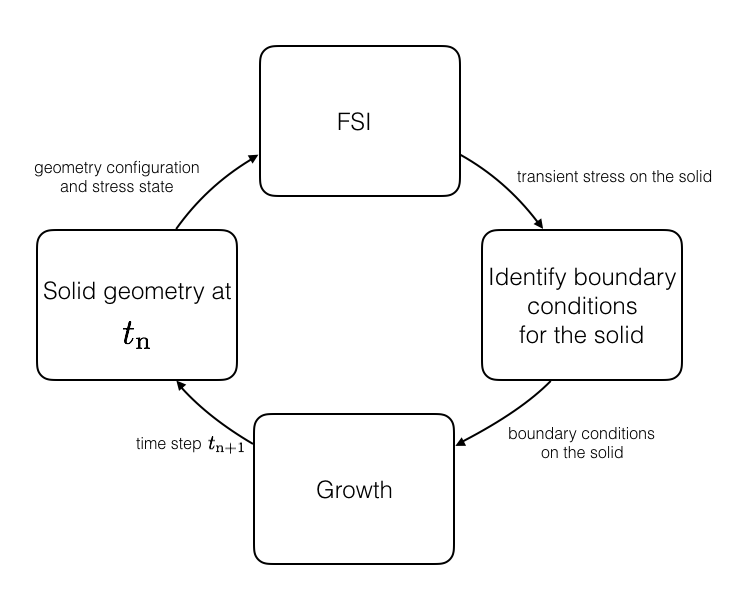
\includegraphics[width=.4\textwidth]{./figs/smallOnLarge.png} % requires the graphicx package
   \caption{Iteration and the information passing in the theory of small on large}
   \label{fig:smallOnLarge}
\end{figure}

The effect of the fluid on the solid is classified as the hydrostatic pressure $p(\bold{X})$ and wall shear stress $\tau(\bold{x})$ which are functions of the undeformed coordinates $\bold{X}$. Let $T$ be the computational period of the FSI process, the average pressure $\bar{p}(\bold{X})$ and wall shear stress $\bar{\boldsymbol{\tau}}(\bold{X})$ can be obtained as:
\begin{subequations}
\begin{align}
\bar{p}(\bold{X}) &= \frac{1}{T}\int_0^T p(\bold{X}) dt\\
\bar{\boldsymbol{\tau}}(\bold{X}) &= \frac{1}{T}\int_0^T \boldsymbol{\tau}(\bold{X}) dt
\end{align}
\end{subequations}